\documentclass[Main.tex]{subfiles} 
\begin{document}

\subsection{Gr�nseflader til eksternt software}
Her beskrives gr�nsefladerne for de software delsystemer, der er blevet udviklet som separate projekter.\\
Der er blevet udviklet en simulator sidel�bende med projektet, da det blev n�dvendigt at have mulighed for at simulere en bus der k�rer p� en rute. Et andet form�l med simulatoren er at g�re det muligt at teste forskellige situationer, der kan forekomme i systemet. 
\subsubsection{Simulator}
N�r simulatoren bliver �bnet vil gr�nsefladen se ud, som vist p� figur \ref{fig:SimulatorViewStart}. Herfra kan der ved "BusNr:" v�lges hvilken busrute, busserne skal k�re p�. Kun ruter med tilknyttede busser vises. "Update speed" bestemmer hvor ofte positionen for busserne skal opdateres i sekunder, hvor '1' er minimumsv�rdien. I "Simulation mode", v�lges der hvilken form for simulation der skal startes, dette kan v�re "Use single bus on route", "Use all busses on chosen route" eller "Use all busses in system".
"Use single bus on route" vil simulere en enkelt bus der k�rer p� den valgte rute, 'Use all busses on chosen route' vil simulere alle de busser der er knyttet til den valgte rute og 'Use all busses in system' vil simulere alle busser i hele systemet p� deres tilknyttede rute. Ved valg af sidste simulerings m�de, er ligemeget hvilken busrute der blev valgt i "BusNr". Under "Bus direction" kan der v�lges om busserne skal k�re i en bestemt eller tilf�ldig retning. Til sidst kan der v�lges hvor hurtig busserne skal k�re. Her er der mulighed for at s�tte hastigheden p� busserne imellem 30 og 1000 km/t. Simulatoren kan nu startes p� to forskellige m�der; Enten hvor busserne alle starter tilf�ldige steder p� deres rute, eller om alle busserne skal starte fra rutens startpunkt.
\begin{figure}[H]
	\centering
	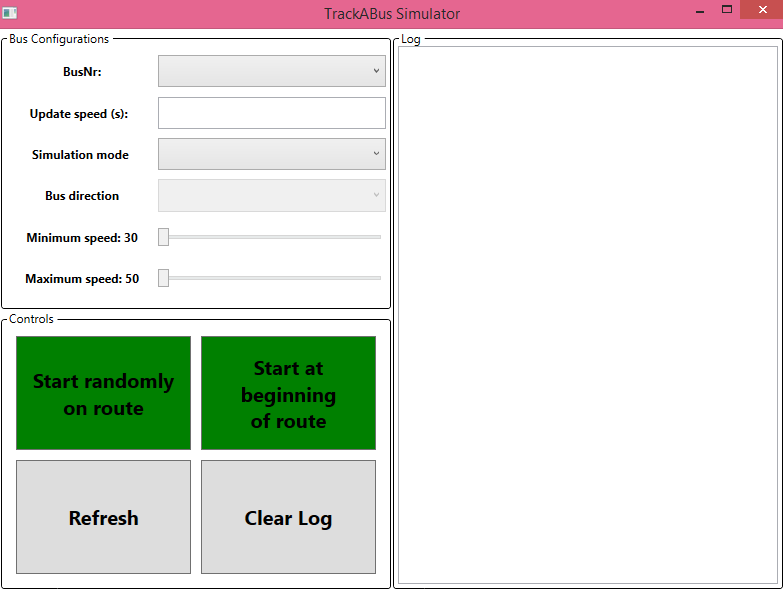
\includegraphics[scale=0.5]{./Diagrammer/Billeder/SimulatorViewStart.png}
	\caption{Gr�nseflade for simulator}
	\label{fig:SimulatorViewStart}
\end{figure}
\noindent
P� figur \ref{fig:SimulatorViewStarted} kan det ses, hvordan gr�nseflade kan se ud efter simulerings start. I h�jre side ses et logvinde, hvor der forekommer opdateringer fra busserne, samt eventuelle fejlbeskeder. De to sidste knapper p� simulatoren, "Refresh" og "Clear Log" bruges henholdsvist til at hente de nyeste ruter fra den distribuerede database, og til at slette alt hvad der st�r i log vinduet.
\begin{figure}[H]
	\centering
	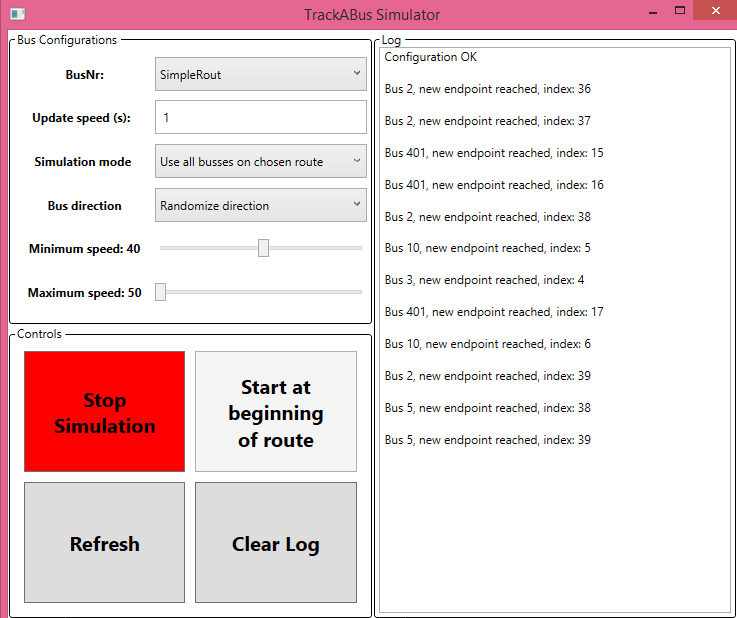
\includegraphics[scale=0.5]{./Diagrammer/Billeder/SimulatorViewStarted.png}
	\caption{Gr�nseflade for simulator efter den er blevet configureret og startet}
	\label{fig:SimulatorViewStarted}
\end{figure}

\end{document}